\documentclass[UTF8]{ctexart}

\usepackage{subfiles}  

%下面的语句, 引入你的头部设置文件
\usepackage{C:/phpStorm_proj/02_myself_ID_EGO/+100_latex_all_math_sel/myPreamble} 
%必须是绝对路径,才能让各个tex在单独编译时使用到

\title{文件名}


%---------------------------------


\begin{document}
	\tableofcontents % 生成目录
	\date{} % 若不写这句, 则默认也会渲染出日期, 所以我们要手动赋空值
	\maketitle  %这行代码, 让你前面的 title, author, date生效
	
	
	
	\section{离散型 : 超几何分布 : \\ $\boxed{
			P\left\{ X=k\text{女} \right\} =\frac{C_{\text{女总数}}^{\text{取}k}C_{\text{男总数}}^{\text{取}n-k\text{人}}}{C_{\text{总}}^{\text{取}n\text{人}}},\ \ k=0,1,...,\min \left\{ n\text{人,女总数} \right\} 
			}$}
	
	超几何分布  (Hypergeometric Distribution), 是统计学上一种离散概率分布. 它描述了: 从有限的N个物件(其中包含M个``指定种类的物件") 中抽出n个物件(不放回). 这n个物件中, 含有k个``指定种类的物件"的概率. \\	
	
	就是: 你从沙子和金粒(金粒=M, 沙子+金粒=N)的混合物中, 捧一把出来(n), 里面含有k个金粒的概率. \\
	
	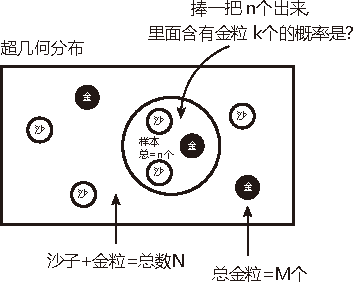
\includegraphics[width=0.45\textwidth]{/0163.pdf} \\
	
	\textbf{简单记忆就是: 从总数N个人中(其中包括了总数M个女人, 则男人数量就是 N-M), 抽出n人, 能取到k个女人的概率.} \\
	
	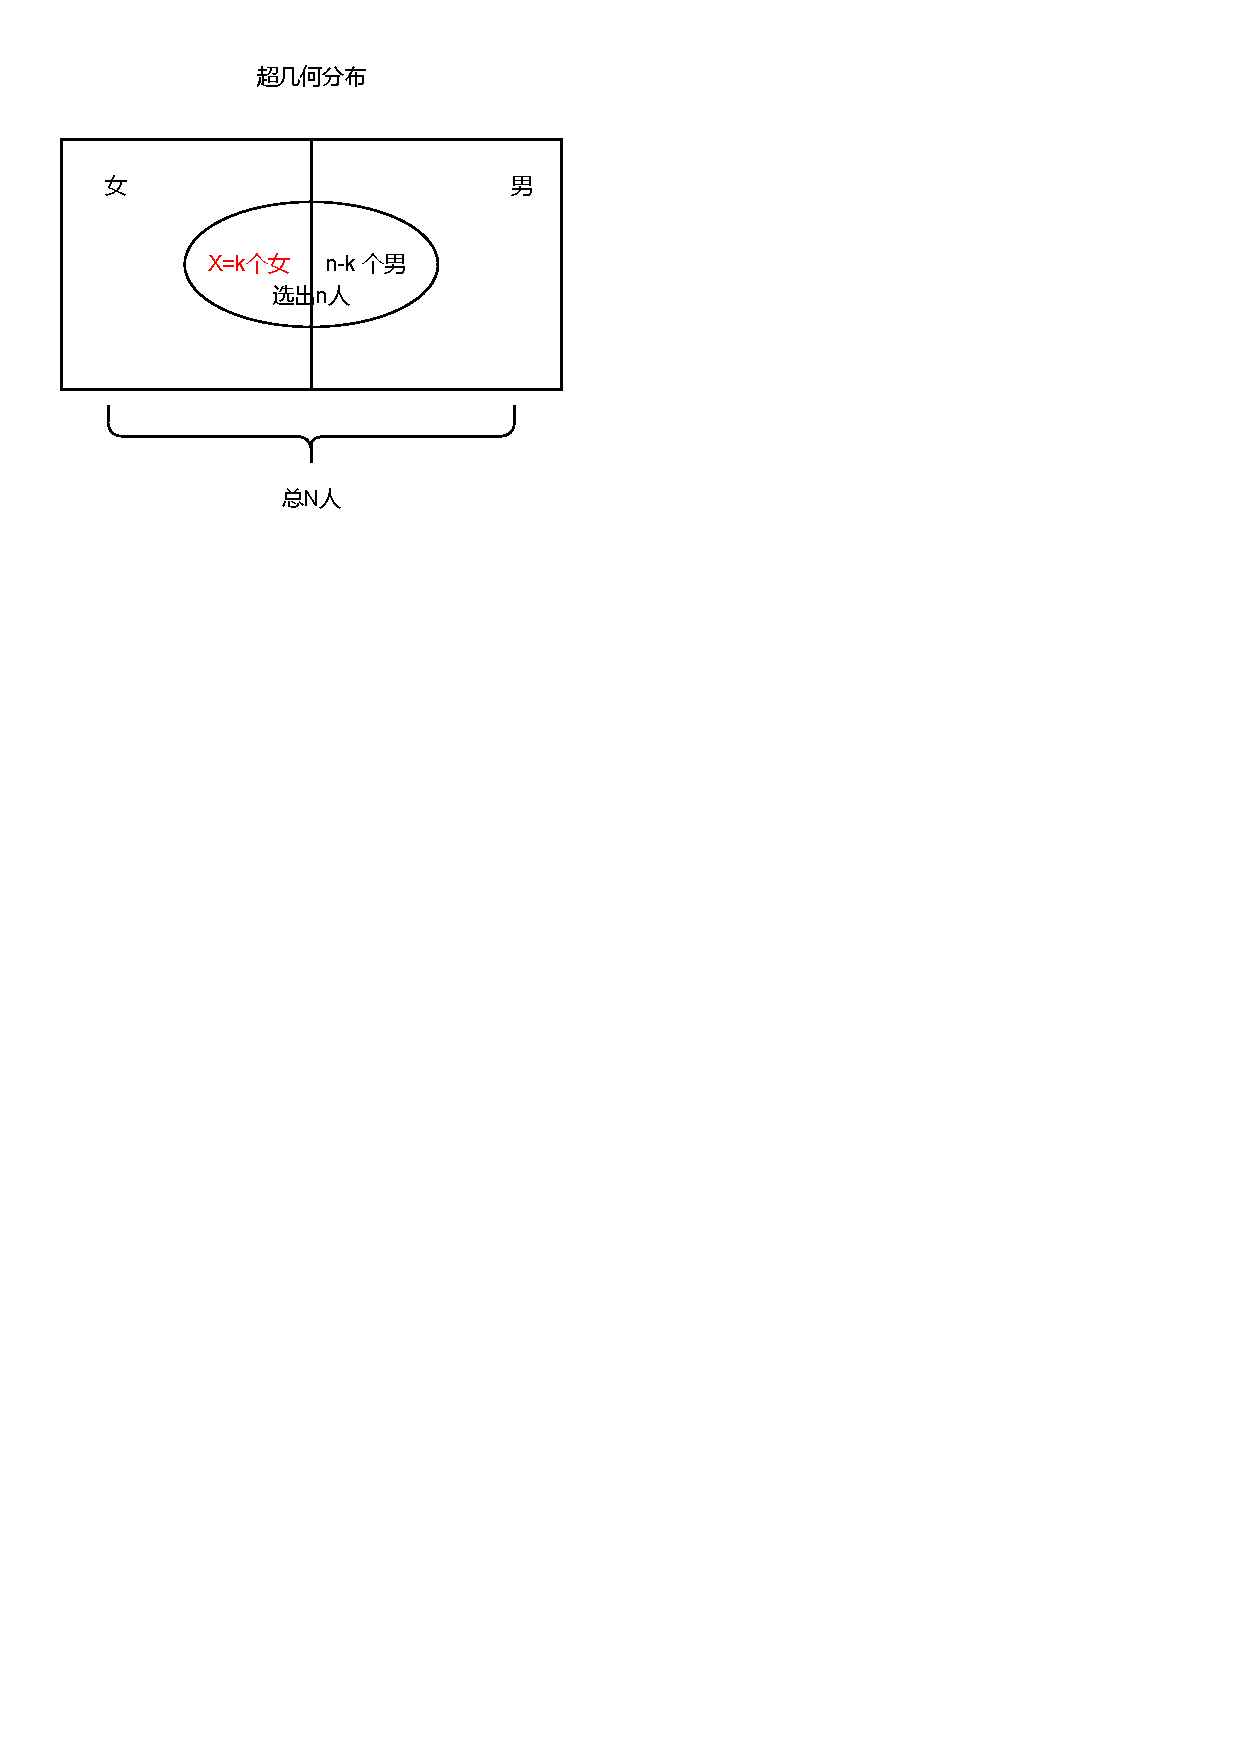
\includegraphics[width=0.5\textwidth]{/0162.pdf} \\
	
	$\boxed{
	P\left\{ X=k\text{女} \right\} =\frac{C_{\text{女人总数}}^{\text{取}k\text{人}}C_{\text{男人总数}}^{\text{取}n-k\text{人}}}{C_{\text{总人数}}^{\text{取}n\text{人}}},\ \ k=0,1,...,\underset{\text{取两者中最小的那个}}{\underbrace{\min \left\{ n\text{人,女人总数} \right\} }}
	}$ \\
	\vspace{1em} 
	
	\begin{myEnvSample}
		有共20人, 其中5女, 15男. 任取4人. 即,  \\
		- X : 表示所抽取的4人中, 女生的人数. 
						
		\begin{align*}  % 支持每行编号. 若不需要编号, 就用 align*环境
	&P\left\{ X=k\text{女} \right\} =\frac{C_{\text{女总}}^{\text{取}k}C_{\text{男数}}^{\text{取}n-k\text{人}}}{C_{\text{总}}^{\text{取}n\text{人}}},\ \ k=0,1,...,\min \left\{ n\text{人,女人总数} \right\}\\
&P\left\{ X=k\text{女} \right\} =\frac{C_{5\text{女}}^{k\text{女}}\cdot C_{15\text{男}}^{4-k\text{女}}}{C_{20}^{4}},\ k=0,1,...,4
		\end{align*}
	
	比如, 所取的4人中, 有2女的概率是 : \\
	$	P\left\{ X=k=2 \right\} =\dfrac{C_{5}^{2}\cdot C_{15}^{4-2}}{C_{20}^{4}}=0.216718	$ \\
	
	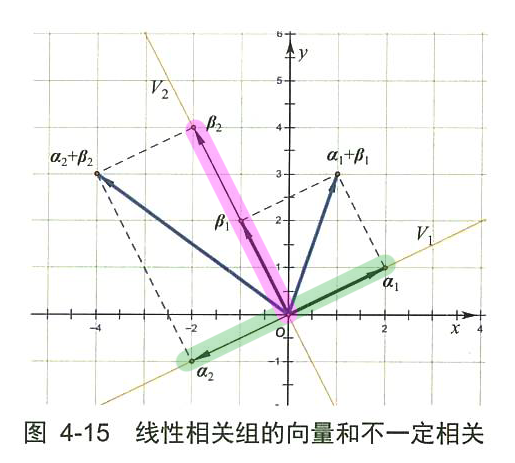
\includegraphics[width=0.9\textwidth]{/0162.png}	
	\end{myEnvSample}
	\vspace{1em} 
	
	
	\begin{myEnvSample}
mathematica 中的``超几何分布"用法: \\
HypergeometricDistribution[n, $n_{succ}, n_{tot}$] \\

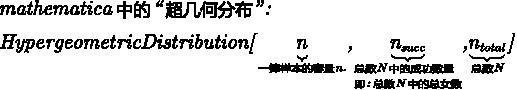
\includegraphics[width=0.8\textwidth]{/0167.pdf} \\
要求:  $0 < n \leq n_{tot}$ 并且 $0 \leq n_{succ} \leq n_{tot} $. \\

例: 共10人, 6女, 4男. \\
抽出5人, 其中有3女的概率是? \\
即: \\
- 总数 nTotal=10 \\
- 总数中的成功数量(即总女) nSuccess= 6 \\
- 一捧的样本容量 n=5 \\

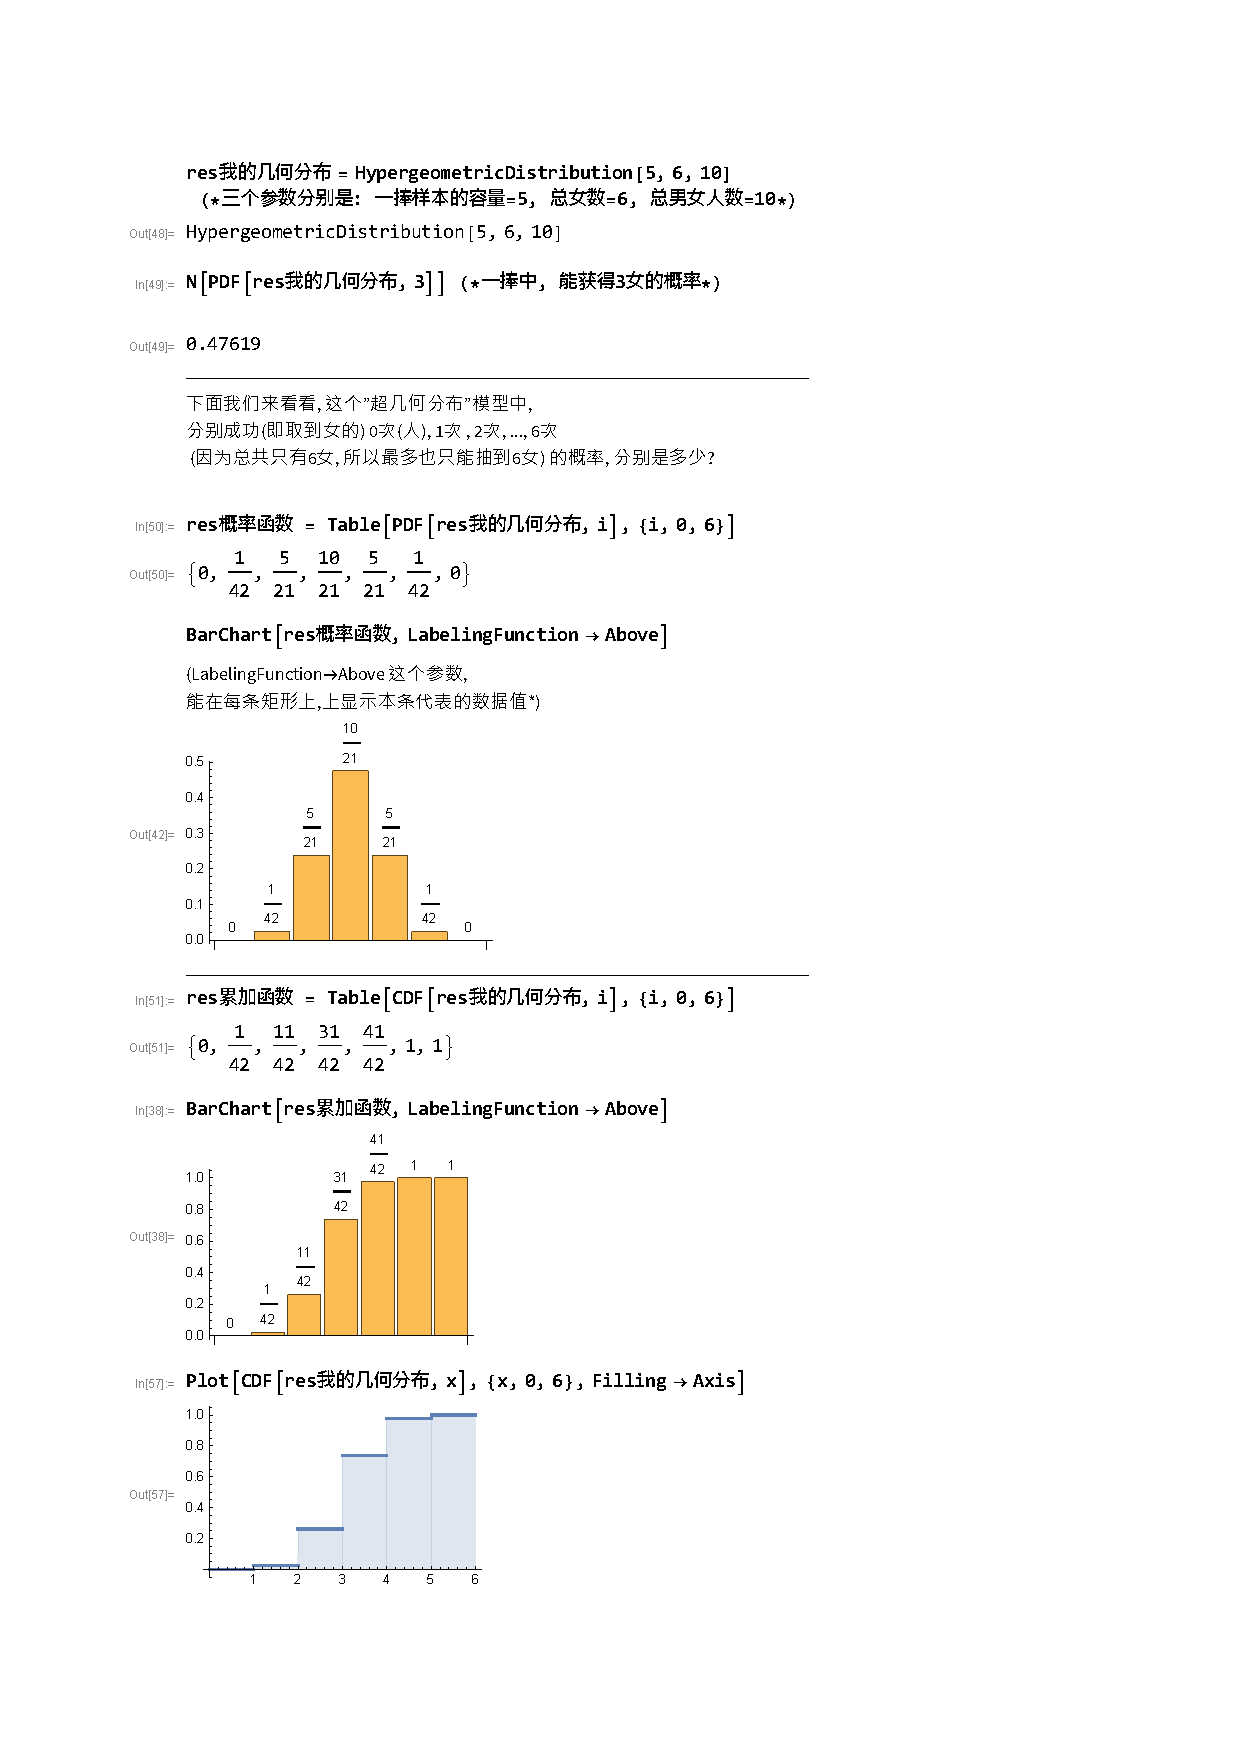
\includegraphics[width=0.85\textwidth]{/0168.pdf} \\
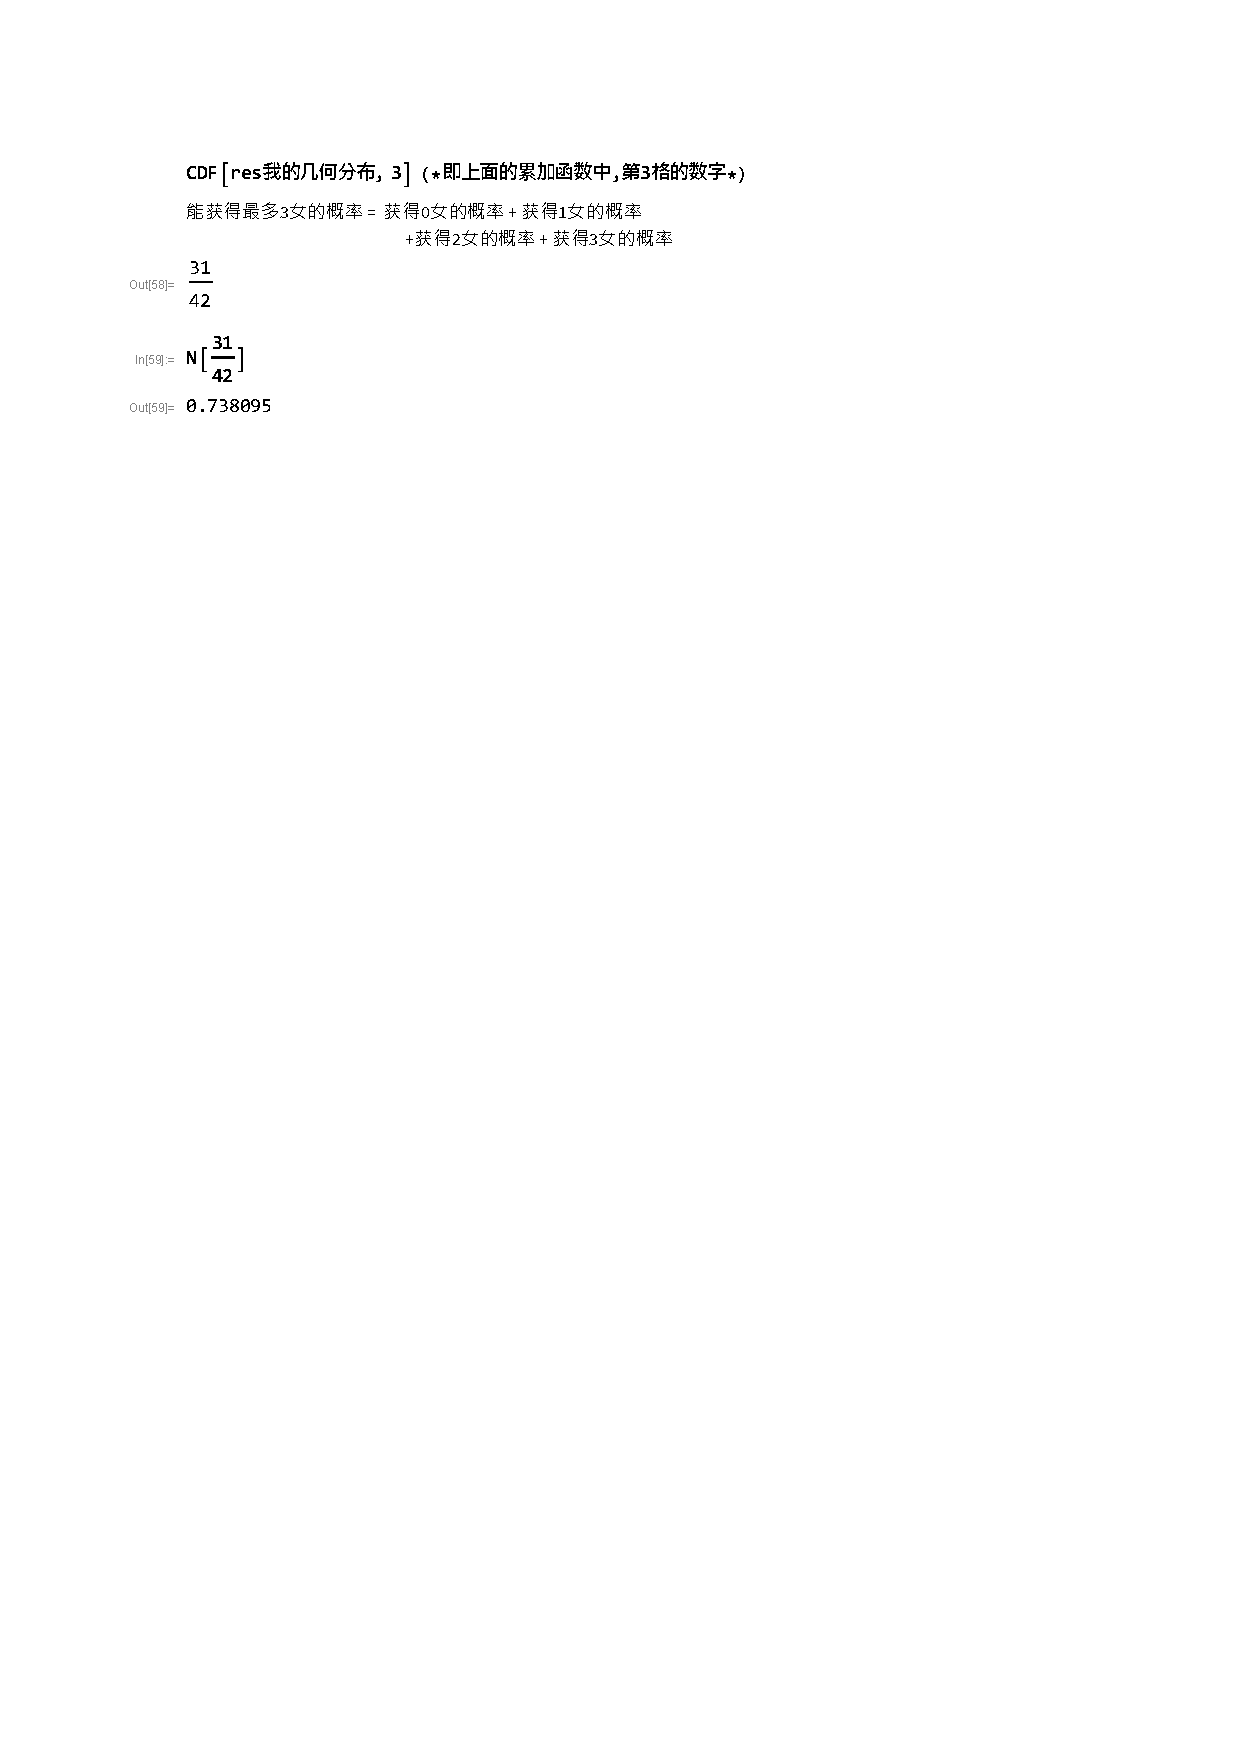
\includegraphics[width=0.8\textwidth]{/0169.pdf} 

	\end{myEnvSample}
	
	
	
	
	\subsection{对于``超几何分布", 当总数N很大, 而所取的n很小时, 即 $\frac{\text{样本中的数量}n}{\text{总数}N}$ 很小时, 我们就能用``二项分布", 来近似该``超几何分布".}
	
	即: $
	P\{X=k\text{女\}}=\underset{\text{超几何分布}}{\underbrace{\frac{C_{\text{总女}}^{\text{取}k\text{女}}\cdot C_{\text{总男}}^{\text{取}n-k=\text{男}}}{C_{\text{总}N}^{\text{取}n}}}}\approx \underset{\text{二项分布}}{\underbrace{C_{n}^{k\text{女}}\cdot \underset{\text{取到}k\text{个女生的概率}}{\underbrace{P^{k\text{女}}}}\cdot \underset{\text{取到}n-k\text{个数量的男生的概率}}{\underbrace{(1-P)^{n-k\text{女}=n\text{中的男数}}}}}}
	$	 \\
	
	
	\begin{myEnvSample}
		有1万粒种子, 发芽率为99\%. 取200粒, 问: 至多有1粒是不发芽的概率? \\
		即: \\
		- 总数N = 10000粒 \\
		- 一捧的样本容量n = 200粒 \\
		- 总数中发芽的, 我们假设它是``沙子", 沙子总数=10000×0.99 \\
		- 总数中不发芽的, 我们假设它是``金子"(注意: 做题中, 我们只对感兴趣的东西, 视为金子. 而无关其是否本身有价值), 金子总数就是 = 10000×0.01 \\
		- X=k : 表示一捧的样本容量200粒中, 金子(即不发芽)的数量k. \\
		
		题目问的是: ``至多有1粒不发芽", 就是有 0粒不发芽(即全发芽), 和1粒不发芽. \\
		
		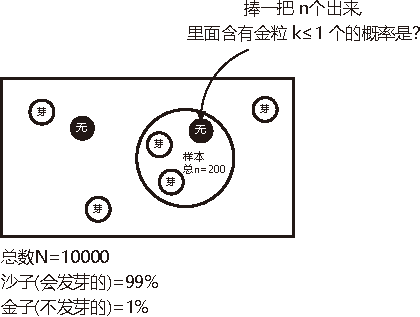
\includegraphics[width=0.55\textwidth]{/0164.pdf} \\
		
		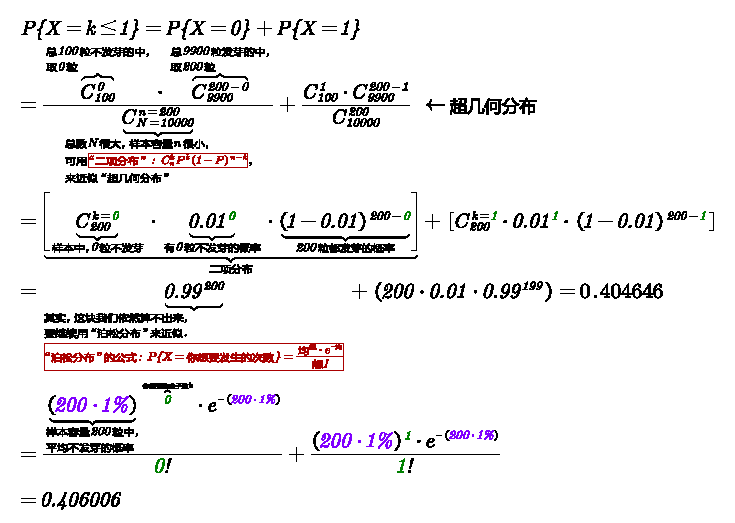
\includegraphics[width=1\textwidth]{/0165.pdf} \\
		
		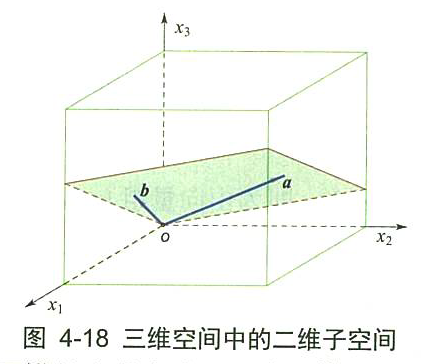
\includegraphics[width=0.55\textwidth]{/0166.png} \\
		
		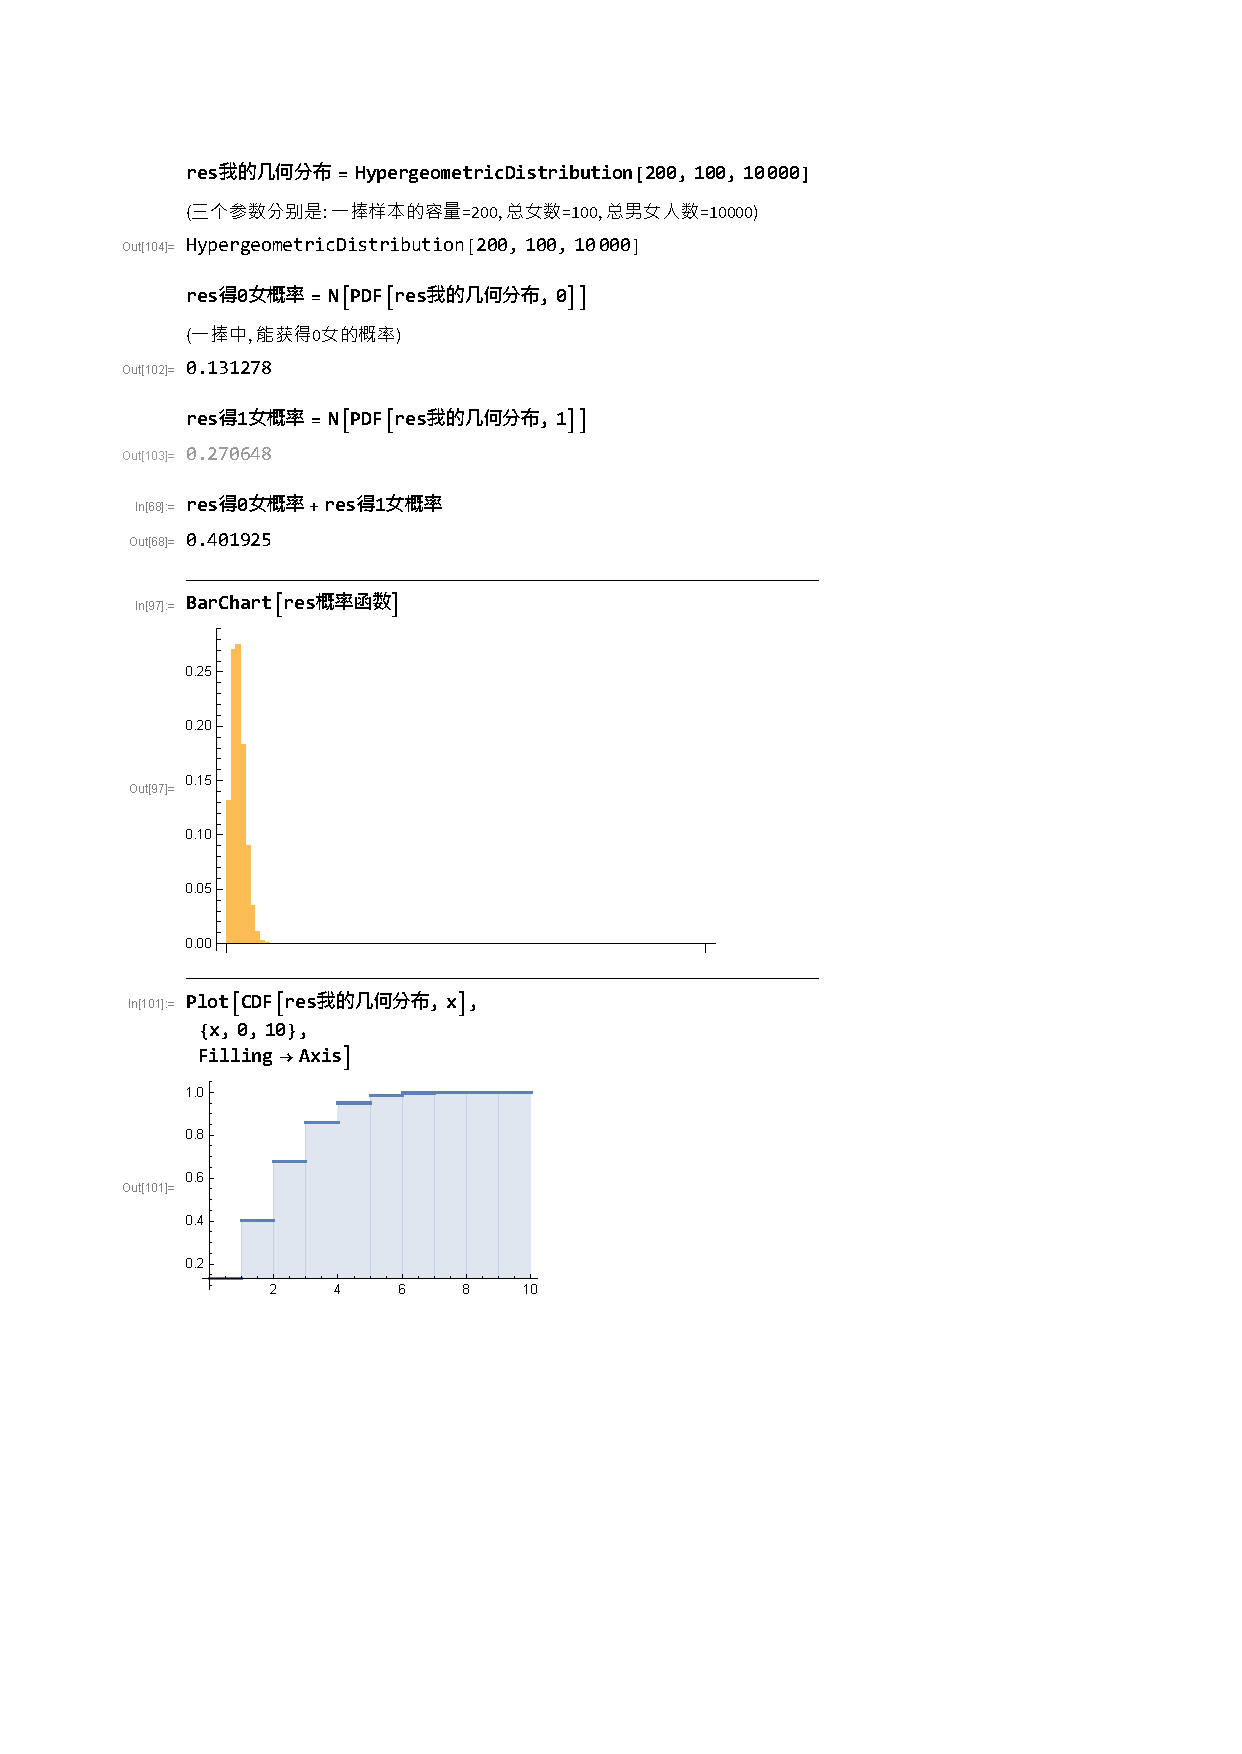
\includegraphics[width=0.9\textwidth]{/0170.pdf}
		
	\end{myEnvSample}



	
	\subsection{对于``二项分布", 当``一捧的样本中的数量n"很大, 而概率P很小时, 就能用``泊松分布"来近似该``二项分布".}
	
\end{document}